\documentclass[tikz,border=15pt]{standalone}
\usepackage{tikz}
\usetikzlibrary{shapes.geometric,arrows.meta,positioning,calc,backgrounds,fit}

\begin{document}
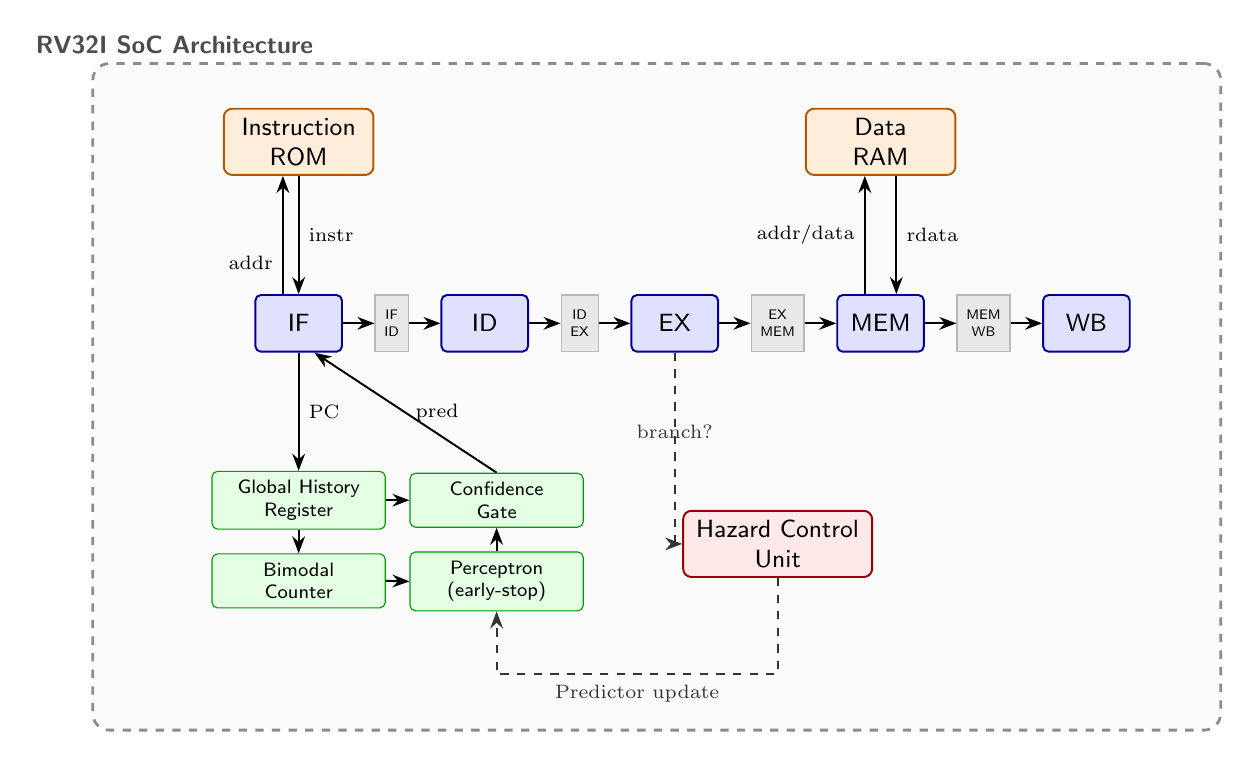
\begin{tikzpicture}[
  font=\sffamily\small,
  every node/.style={align=center},
  %% ─── 節點樣式定義 ────────────────────────────────────────────────
  stage/.style={
    draw=blue!60!black, fill=blue!12, rounded corners=2pt,
    minimum width=1.10cm, minimum height=0.72cm, line width=0.7pt},
  pipereg/.style={
    draw=gray!55, fill=gray!18,
    minimum width=0.30cm, minimum height=0.72cm, line width=0.5pt, font=\sffamily\tiny},
  memblk/.style={
    draw=orange!70!black, fill=orange!14, rounded corners=3pt,
    minimum width=1.9cm, minimum height=0.70cm, line width=0.7pt},
  ctrlbox/.style={
    draw=red!60!black, fill=red!9, rounded corners=3pt,
    minimum width=2.4cm, minimum height=0.70cm, line width=0.7pt},
  sub/.style={
    draw=green!60!black, fill=green!10, rounded corners=2pt,
    minimum width=2.2cm, minimum height=0.5cm, font=\sffamily\scriptsize},
  arrow/.style={->, >=Stealth, line width=0.7pt},
  darrow/.style={->, >=Stealth, dashed, line width=0.7pt, color=black!80}
]

  %% ─── 1. 流水線階段與暫存器 (稍微拉開間距讓佈局呼吸) ───────────────
  \node[stage] (IF) {IF};
  \node[pipereg, right=0.4cm of IF] (IFID) {IF\\ID};
  \node[stage, right=0.4cm of IFID] (ID) {ID};
  \node[pipereg, right=0.4cm of ID] (IDEX) {ID\\EX};
  \node[stage, right=0.4cm of IDEX] (EX) {EX};
  \node[pipereg, right=0.4cm of EX] (EXMEM) {EX\\MEM};
  \node[stage, right=0.4cm of EXMEM] (MEM) {MEM};
  \node[pipereg, right=0.4cm of MEM] (MEMWB) {MEM\\WB};
  \node[stage, right=0.4cm of MEMWB] (WB) {WB};

  %% ─── 2. 存儲子系統 (Memories) ────────────────────────────────────
  \node[memblk, above=1.5cm of IF] (ROM) {Instruction\\ROM};
  \node[memblk, above=1.5cm of MEM] (RAM) {Data\\RAM};

  %% ─── 3. 預測器子模組 (對齊左半邊 IF 與 ID 區域) ──────────────────
  \node[sub, below=1.5cm of IF] (GHR) {Global History\\Register};
  \node[sub, right=0.3cm of GHR] (Conf) {Confidence\\Gate};
  \node[sub, below=0.3cm of GHR] (Bimodal) {Bimodal\\Counter};
  \node[sub, below=0.3cm of Conf] (Percep) {Perceptron\\(early-stop)};

  %% ─── 4. 冒險控制單元 (移至右半邊 EXMEM 下方，徹底避開碰撞) ────────
  \node[ctrlbox, below=2.0cm of EXMEM] (Hazard) {Hazard Control\\Unit};

  %% ─── 5. 訊號佈線 (Routing & Connections) ─────────────────────────
  % ROM 提取指令
  \draw[arrow] (ROM.south) -- (IF.north) node[midway, right, font=\scriptsize] {instr};
  \draw[arrow] ([xshift=-0.2cm]IF.north) -- ++(0,0.4) -| ([xshift=-0.2cm]ROM.south) node[pos=0.2, left, font=\scriptsize] {addr};

  % RAM 存取數據
  \draw[arrow] ([xshift=-0.2cm]MEM.north) -- ([xshift=-0.2cm]RAM.south) node[midway, left, font=\scriptsize] {addr/data};
  \draw[arrow] ([xshift=0.2cm]RAM.south) -- ([xshift=0.2cm]MEM.north) node[midway, right, font=\scriptsize] {rdata};

  % 流水線主資料流
  \foreach \s/\r in {IF/IFID, IFID/ID, ID/IDEX, IDEX/EX, EX/EXMEM, EXMEM/MEM, MEM/MEMWB, MEMWB/WB} {
    \draw[arrow] (\s) -- (\r);
  }

  % 預測器外圍訊號
  \draw[arrow] (IF.south) -- (GHR.north) node[midway, right, font=\scriptsize] {PC};
  \draw[arrow] (Conf.north) -- ([xshift=0.2cm]IF.south) node[midway, right, font=\scriptsize] {pred};
  
  % 預測器內部資料流拓撲
  \draw[arrow] (GHR.east) -- (Conf.west);
  \draw[arrow] (GHR.south) -- (Bimodal.north);
  \draw[arrow] (Bimodal.east) -- (Percep.west);
  \draw[arrow] (Percep.north) -- (Conf.south);

  % 冒險控制與權重更新訊號 (虛線)
  % 修正 1：branch? 訊號從 EX 直角向下後向右走入 Hazard 左側
  \draw[darrow] (EX.south) |- (Hazard.west) node[pos=0.25, above, font=\scriptsize] {branch?};
  
  % 修正 2：Predictor update 從 Hazard 底部出發，從下方安全繞過 Predictor 外框，回到 Perceptron 底部
  \draw[darrow] (Hazard.south) |- ([yshift=-0.8cm]Percep.south) node[pos=0.75, below, font=\scriptsize] {Predictor update} -- (Percep.south);

  %% ─── 6. 封裝背景框 (Background Grouping Boxes) ───────────────────
  \begin{scope}[on background layer]
    % Predictor Box
    \node[draw=green!50!black, dashed, fill=green!5, 
          rounded corners=4pt, line width=0.8pt, inner sep=10pt,
          fit=(GHR) (Conf) (Bimodal) (Percep),
          label={[font=\sffamily\scriptsize\bfseries, green!60!black, inner sep=2pt]above left:Predictor}
         ] (predgrp) {};

    % Pipelined CPU Core Box
    \node[draw=blue!55!black, fill=blue!3, 
          rounded corners=5pt, line width=1pt, inner sep=16pt,
          fit=(IF) (WB) (Hazard) (predgrp),
          label={[font=\sffamily\footnotesize\bfseries, blue!70!black, inner sep=3pt]above right:Pipelined CPU Core}
         ] (cpucore) {};

    % RV32I SoC Box
    \node[draw=black!45, dashed, fill=gray!3, 
          rounded corners=6pt, line width=1pt, inner sep=16pt,
          fit=(ROM) (RAM) (cpucore),
          label={[font=\sffamily\small\bfseries, black!70, inner sep=3pt]above left:RV32I SoC Architecture}
         ] (soc) {};
  \end{scope}

\end{tikzpicture}
\end{document}